\documentclass[runningheads]{llncs}

\usepackage[T1]{fontenc}
\usepackage{amsmath,amssymb}
\usepackage{booktabs}
\usepackage{graphicx}
\usepackage{xcolor}
\usepackage{hyperref}
\usepackage{pgfplots}
\pgfplotsset{compat=1.18}
\renewcommand\UrlFont{\color{blue}\rmfamily}
\urlstyle{rm}
\graphicspath{{figures/}}
\emergencystretch=1.5em

\begin{document}

\title{Stress-Testing Product-Gated Clustering and Bounded Priority
Ranking for Flood-Rescue Reports}
\titlerunning{Stress-Testing Flood-Rescue Report Clustering and Ranking}

\author{Anonymous Authors}
\authorrunning{Anonymous Authors}
\institute{Anonymous for review}

\maketitle

\begin{abstract}
Operational flood streams contain duplicate, incomplete, and adversarial
reports, while clustering and priority scores are often evaluated without
measuring their scheduling consequences. We audit a fail-closed batch
pipeline in which observable reports form a sparse graph, unresolved reports
go to review, duplicate families feed a bounded score, and evaluator-only
truth is joined after predicted-cluster scheduling. The clustering benchmark
contains 80 synthetic runs from generator 3.0.0: additive Louvain has mean
ARI $0.9191$, product Leiden $0.9165$, and product Louvain $0.9072$.
Product minus independently tuned additive is $-0.0118$ (bootstrap 95\% CI
$[-0.0226,-0.0024]$), but its Holm-adjusted test is not significant
($p=.2560$). A matched-density comparison reverses the point estimate but is
also inconclusive. In a separate candidate-4.1 bundle, the revised score
has NDCG@5 $0.6669$ versus $0.6763$ for a random comparator and does not
show a general alignment advantage; exact duplicates are invariant but
coordinated high-confidence campaigns remain a failure mode. Dispatch
results similarly show no general benefit over the legacy score and a clear
cost relative to nearest-first. These are synthetic, within-generator
diagnostics: boundedness and clustering accuracy do not establish source
authenticity, policy validity, field benefit, or deployment readiness.
\keywords{Flood rescue \and Graph clustering \and Synthetic stress test \and
Priority ranking \and Negative results.}
\end{abstract}

\section{Introduction and Related Work}

During emergencies, crisis streams mix repeated reports of one event with
nearby but distinct events, missing fields, and nonincident noise. Social-sensor
and emergency-message research addresses volume, verification, and event
extraction~\cite{sakaki2010earthquake}.
CrisisMMD and FloodNet capture useful disaster modalities, although FloodNet
is an aerial post-flood scene-understanding dataset rather than a multimodal
report stream~\cite{alam2018crisismmd,rahnemoonfar2021floodnet}. These resources
do not jointly provide physical-incident linkage, rescue priority, and field
dispatch outcomes.

\paragraph{Social sensing and event extraction.}
Social-media users can act as real-time sensors~\cite{sakaki2010earthquake},
but the usual endpoint is event detection or classification rather than the
consequences of sending a field resource to a predicted incident.

\paragraph{Consolidation and clustering.}
Graph community detection with Louvain or Leiden
\cite{blondel2008louvain,traag2019leiden}, and density methods such as DBSCAN
and HDBSCAN~\cite{ester1996dbscan} offer plausible consolidation mechanisms.
Multiplicative spatial--range
terms occur in bilateral filtering~\cite{tomasi1998bilateral}; we adapt that
structure to a product graph, while testing the exact gate and its bounds here.

\paragraph{Humanitarian logistics and dispatch.}
Relief-routing models expose competing equity, efficacy, and efficiency
objectives~\cite{gralla2014review}.
We use this perspective to motivate a bounded priority ranking, but boundedness
is not an expert-endorsed policy. A key gap is propagation of false splits,
merges, and noise into a scheduler that cannot consult incident truth.

We address these gaps with a fail-closed batch pipeline: reports with
observable location and time enter a sparse graph, incomplete reports go to
manual review, duplicate families feed a bounded ranking, and evaluator-only
truth joins after predicted-cluster scheduling. We ask:
(RQ1) does independently selected product composition improve clustering over
additive composition? (RQ2) does the duplicate-aware score align with an
independently generated benefit under report-level stress tests? (RQ3) how do
predicted split, merge, and noise errors propagate into dispatch? The questions
use two explicitly separated artifact bundles.

The contributions are (i) an observable-only pipeline with explicit review and
evaluator boundaries; (ii) auditable threshold statements and a proposed
duplicate-aware score; and (iii) a paired diagnostic reporting clustering,
ranking, dispatch, and adverse results. The evidence remains synthetic and
within-generator, so the artifact is not a validated rescue policy.

\section{Observable Pipeline and Methods}

Figure~\ref{fig:pipeline} fixes the information boundary. Observable report
fields flow through graph construction, ranking, and a batch scheduler.
Missing location or timestamp routes a report to review. Incident identity,
benefit, deadline, and harm are stored separately and join only after a
schedule exists.

\begin{figure}[t]
\centering

\includegraphics[width=\textwidth]{pipeline_v2.pdf}
\caption{Observable pipeline (solid), manual-review path (orange), and
evaluator-only truth join (dashed). The scheduler receives predicted
clusters, never incident truth.}
\label{fig:pipeline}
\end{figure}

\subsection{Report Attributes and Missingness}

Each report is represented by the compact tuple
\[
r_i=(L_i,T_i,F_i,E_i,N_i,V_i,Q_i),
\]
where $L_i$ is a GPS location and $T_i$ is the observable report timestamp
(``created\_at''). Flood evidence $F_i$ and urgency evidence $E_i$ are in
$[0,1]$; $N_i\in\mathbb{Z}_{\geq0}$ is the reported trapped-person count;
$V_i\geq0$ is a vulnerability-evidence value; and $Q_i\in[0,1]$ is a
provenance/confidence heuristic. $Q_i$ is not a calibrated probability of
truth. The implementation also carries observable support fields such as
image presence, source type, province, and missing-field flags; these support
$Q_i$ and duplicate fingerprints but are not additional latent labels.

The score $Q_i$ is computed from observable image presence and a capped count
$n_i^{\rm corrob}$ of nearby corroborating payloads using the proposed
heuristic
\[
\begin{aligned}
Q_i&=\operatorname{sigmoid}\!\left(b_0+b_1\mathbf{1}\{\text{image}_i\}
 +b_2\log(1+n_i^{\rm corrob})\right),\\[-1mm]
&(b_0,b_1,b_2)=(-.2,1.4,.9).
\end{aligned}
\]
Here $\operatorname{sigmoid}(x)=(1+e^{-x})^{-1}$.
This is a pipeline rule, not a calibrated truth model. No independent receipt
timestamp or source family is assumed. The admission indicator
$a_i=\mathbf{1}\{L_i,T_i\text{ observed}\}$, the masks
$I_F(i,j),I_E(i,j)$, and $m_{ij}=I_F(i,j)+I_E(i,j)$ are derived pairwise
quantities; hence $a_i a_j=0$ prevents an edge whose geographic or temporal
separation is undefined. Missing $F$ or $E$ is not zero-imputed. Following the general
missing-variable kernel problem~\cite{smola2005missing}, we use the
fail-closed construction
\[
C_{ij}=\frac{m_{ij}}{2}\exp\!\left[-I_F(i,j)\frac{|F_i-F_j|}{\tau_F}
-I_E(i,j)\frac{|E_i-E_j|}{\tau_E}\right],\qquad
C_{ij}=0\ \text{if }m_{ij}=0.
\]
Thus complete context gives the usual exponential similarity, one shared
field gives at most one half, and no shared field gives no inferred
agreement. In particular, when $m_{ij}=2$,
$C_{ij}=\exp[-|F_i-F_j|/\tau_F-|E_i-E_j|/\tau_E]$. All RQ1 reports contain
$F$ and $E$, so the evaluated RQ1 graph
uses the complete-data reduction; missingness is a specified, not an
empirically claimed, extension.

\subsection{Similarity Graph and Derived Bounds}

For Haversine distance $d_{ij}$ and time difference $\Delta t_{ij}$, define
the Gaussian affinity~\cite{ng2001spectral} and normalized temporal decay
\cite{zhou2013triggering}
\begin{align}
G_{ij}&=\exp[-d_{ij}^{2}/(2\sigma^2)],&
T_{ij}&=\exp[-\Delta t_{ij}/\tau_t],\nonumber\\
w^\times_{ij}&=a_i a_jG_{ij}(\beta T_{ij}+\gamma C_{ij}),&
w^+_{ij}&=a_i a_j(\alpha G_{ij}+\beta T_{ij}+\gamma C_{ij}).
\label{eq:similarities}
\end{align}
The exponential form is a precedent, not a claim that the complete
missingness-aware expression is copied from prior work~\cite{billot2008exponential}.
The product is a spatial gate motivated by spatial--range products such as
bilateral filtering~\cite{tomasi1998bilateral}; both compositions and all
weights here are defined by this paper.

The implementation uses a common spatial candidate pool, an empirical
nonzero-weight quantile, strict above-threshold edges, endpoint top-$k$
retention, and Louvain or Leiden. Product and additive candidates are tuned
independently; their comparison is therefore a pipeline comparison. All
scales are positive and all composition weights are nonnegative.

\begin{theorem}[Product edge localization]
Let $B=\beta+\gamma>0$. If a product edge with threshold $0<\theta<B$ is
retained, then
$d_{ij}<\sigma\sqrt{2\log(B/\theta)}$. For $\theta\geq B$ the strict
retained set is empty.
\end{theorem}
\begin{proof}
Because $a_ia_j\leq1$ and $T_{ij},C_{ij}\leq1$,
$w^\times_{ij}\leq B\exp[-d_{ij}^{2}/(2\sigma^2)]$. Combining this bound
with $\theta<w^\times_{ij}$ and taking logarithms gives the result.
\end{proof}

\begin{corollary}[Conditional component bound]
If a retained product component has observed unweighted hop diameter $h<\infty$,
then its geographic diameter is less than
$h\sigma\sqrt{2\log(B/\theta)}$.
\end{corollary}
This is a conditional post-hoc statement: the pipeline does not control $h$.
For the additive form, a finite geographic cutoff exists only when
$B<\theta<B+\alpha$, with radius
$\sigma\sqrt{2\log(\alpha/(\theta-B))}$. These are deductions from the
weight definitions, not empirical performance guarantees.

\subsection{Duplicate-Aware Bounded Ranking}

Exact duplicate payloads share a canonical fingerprint. Near duplicates are
joined by deterministic connected components under the observable envelope;
this transitive rule is not complete linkage. Let $g$ index the resulting
evidence families. For the current candidate source snapshot, the revised
estimator uses confidence-gated family maxima and avoids treating overlapping
reports as disjoint people. Write
$\widetilde N_i=\min(N_i,N_{\rm ref})$ and
$\widetilde V_i=\min(V_i,V_{\rm cap})$ for the nonnegative clipped claims:
\begin{align}
\bar E&=\frac{\sum_g\max_{i\in g}Q_iE_i}
 {\max(1,\sum_g\max_{i\in g}Q_i)},&
\bar F&=\max_{g,i\in g}Q_iF_i,\nonumber\\
\bar N&=\min\!\left(1,\frac{\log(1+\max_{g,i\in g}Q_i\widetilde N_i)}
 {\log(1+N_{\rm ref})}\right),&
\bar V&=\max_{g,i\in g}Q_i\widetilde V_i,\nonumber\\
P&=\left[1+(\mu-1)\tanh(\bar V/s)\right]
 (\omega_E\bar E+\omega_F\bar F+\omega_N\bar N).
\label{eq:priority}
\end{align}
The candidate source snapshot associated with the RQ2/RQ3 artifacts specifies
$\omega=(.34,.33,.33)$, $\mu=2$, $s=10$, $N_{\rm ref}=500$, and
$V_{\rm cap}=50$; the Colab configuration audit must confirm these values
against the locked bundle before submission. The formula is a proposed
policy heuristic: maxima limit duplicate multiplicity, the logarithm
compresses heavy-tailed demand, clipping bounds individual evidence, and the
hyperbolic tangent saturates vulnerability amplification. Reliability-aware
truth discovery motivates using $Q_i$ but does not derive these maxima
\cite{wang2012truth}. Transformation, normalization, and weights require
sensitivity and expert validation~\cite{tate2012vulnerability,gralla2014review}.

\section{Experimental Design}

\paragraph{Two artifact bundles.}
RQ1 uses generator 3.0.0, seeds 1--80, and 20 development, 20 calibration,
and 40 benchmark-test runs. The last 40 are a benchmark split within the
same generator regime, not an unseen OOD test. RQ2 and RQ3 use candidate
generator 4.1.0, test seeds 3000--3039, and bundle SHA
\texttt{a7c7a3f7...f2d7e1}; their manifests are stored with the result CSVs.
Both bundles are geographically anchored to the Copernicus EMSR848 Central
Viet Nam flood activation; incidents, reports, duplicates, campaigns, and
labels remain synthetic.

\paragraph{RQ1 clustering.}
The calibration notebook selects each composition independently by mean ARI,
then standard deviation and canonical configuration JSON. Product uses
$\sigma=700$ m, $\tau_t=60$ min, quantile $.90$, and $k=8$; additive uses
$\alpha=1$, the same scales and $k$, and quantile $.95$. The common candidate
pool and grid make the comparison reproducible but not causal. ARI is primary;
NMI, pair F1, diameter, edge fraction, and operational-noise fields are
descriptive. Paired differences use 10,000 bootstrap resamples, Wilcoxon
tests, and Holm correction~\cite{hubert1985comparing}. K-means is the
coordinate comparator~\cite{macqueen1967some}.

\paragraph{RQ2 score isolation.}
The evaluator generates an independent relevance signal from latent incident
benefit and computes NDCG@5, Spearman correlation, and top-five overlap. It
uses oracle incident grouping only to isolate score behavior; inference sees
observable reports only. Exact duplicates, near duplicates, contradictions,
missingness, and coordinated campaigns are injected as stress scenarios.

\paragraph{RQ3 error propagation.}
The scheduler receives Product, matched-density Additive, or oracle partitions
and compares revised, legacy, FIFO, nearest-first, equity-aging, and workload
smoothing policies. The conservative evaluator permits one destination per
incident, charges split trips and fake-only dispatches, and scores unserved
incidents at 480 minutes. Paired effects use the CSV column \texttt{mean}, whose
positive direction is already oriented as better for the candidate; raw
lower-is-better differences have the opposite sign.

\section{Results}

\begin{table}[t]
\centering\scriptsize
\caption{RQ1 benchmark-test summary (40 runs). Intervals are bootstrap 95\%
CI low--high; diameter is descriptive.}
\label{tab:clustering-results}
\begin{tabular}{lccr}
\toprule
Method & ARI [95\% CI] & Pair F1 & Mean diam. (km)\\
\midrule
Additive Louvain & .9191 [.8995,.9381] & .9247 & .3477\\
Product Leiden & .9165 [.8979,.9351] & .9223 & .3547\\
Convex Louvain & .9135 [.8940,.9320] & .9195 & .3547\\
Product Louvain & .9072 [.8864,.9271] & .9138 & .3585\\
Coordinate K-means & .8176 [.7976,.8384] & .8292 & .2977\\
HDBSCAN & .5205 [.4565,.5811] & .5787 & 1.2527\\
\bottomrule
\end{tabular}
\end{table}

Additive Louvain has the highest mean ARI. Product minus independently tuned
additive is $-0.01184$ with CI $[-0.02257,-0.00240]$, 9 wins, 19 ties, and
12 losses; raw $p=.0987$ and Holm $p=.2560$. Product minus matched-density
additive is $+0.00989$ with CI $[-0.00100,0.02082]$ and Holm $p=.2560$.
Product Leiden versus Product Louvain has Holm $p=.1120$. Thus neither
composition advantage is established. Product and additive have nearly equal
retained edge fractions ($.03011$ and $.03021$) and mean degrees (9.90 and
9.94), supporting the matched-density interpretation. Product has zero fake
absorption and zero fake rejection but 16.49\% false destinations: fakes avoid
genuine destinations while still forming fake-only destinations, so this is
not misinformation robustness.

\begin{figure}[t]
\centering
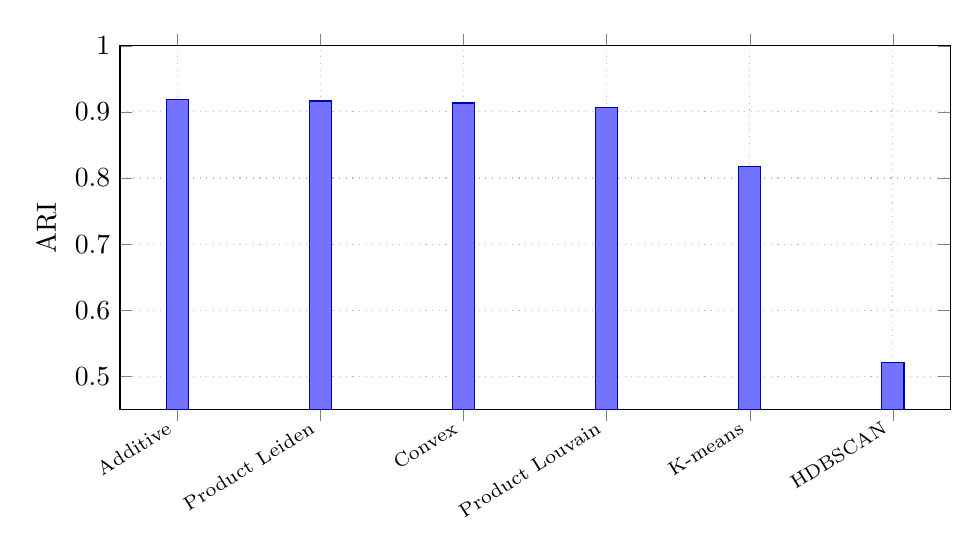
\begin{tikzpicture}
\begin{axis}[
  width=\textwidth,
  height=6.2cm,
  ybar,
  bar width=8pt,
  symbolic x coords={Additive,Product Leiden,Convex,Product Louvain,K-means,HDBSCAN},
  xtick=data,
  xticklabel style={font=\scriptsize,rotate=32,anchor=east},
  ylabel={ARI},
  ymin=0.45,
  ymax=1.0,
  ytick={0.5,0.6,0.7,0.8,0.9,1.0},
  grid=major,
  grid style={dotted,gray!50},
  enlarge x limits=0.08,
]
\addplot+[fill=blue!55,draw=blue!70!black]
  coordinates {
    (Additive,0.9191)
    (Product Leiden,0.9165)
    (Convex,0.9135)
    (Product Louvain,0.9072)
    (K-means,0.8176)
    (HDBSCAN,0.5205)
  };
\end{axis}
\end{tikzpicture}
\caption{RQ1 benchmark-test ARI means. The plotted values are the same summary
used in Table~\ref{tab:clustering-results}; bootstrap intervals remain reported
in the table.}
\label{fig:rq1-ari}
\end{figure}

\begin{table}[t]
\centering\scriptsize
\caption{Headline RQ2/RQ3 results from the candidate-4.1 artifacts. For paired
rows, a positive effect means the revised candidate is better; negative effects
are therefore adverse.}
\label{tab:stress-results}
\begin{tabular}{llrr}
\toprule
Question & Contrast and metric & Effect & Holm $p$\\
\midrule
RQ2 & Revised NDCG@5 (absolute) & .6669 & --\\
    & Random NDCG@5 (absolute) & .6763 & --\\
    & Revised $-$ legacy NDCG@5 & +.0121 & .5882\\
    & Exact-duplicate priority drift & 0 & --\\
    & Coordinated-campaign drift & .1688 & --\\
RQ3 & Revised $-$ legacy, Product harm & $-14.34$ & .675\\
    & Revised $-$ legacy, Product deadline & +.0188 & .160\\
    & Revised $-$ nearest, Product harm & $-69.88$ & $1.8\times10^{-7}$\\
    & Revised $-$ nearest, Product deadline & $-.1771$ & $3.0\times10^{-15}$\\
    & Product $-$ matched Additive harm & $-18.34$ & .000151\\
\bottomrule
\end{tabular}
\end{table}

RQ2 shows no general alignment benefit: revised NDCG@5 is .6669 (CI
[.6306,.7018]), below population-only (.6709) and random (.6763), and no
comparator contrast is Holm-significant. Revised priority is invariant to
2$\times$, 5$\times$, and 10$\times$ exact duplication. Near duplicates and
some missingness scenarios improve over legacy, but a coordinated
high-confidence campaign produces drift .1688 and false-priority lift .8828;
revised drift is worse than legacy ($\Delta=-.1379$, Holm
$p\approx9.1\times10^{-12}$). Boundedness is therefore not a guarantee of
ranking reliability.

\begin{figure}[t]
\centering
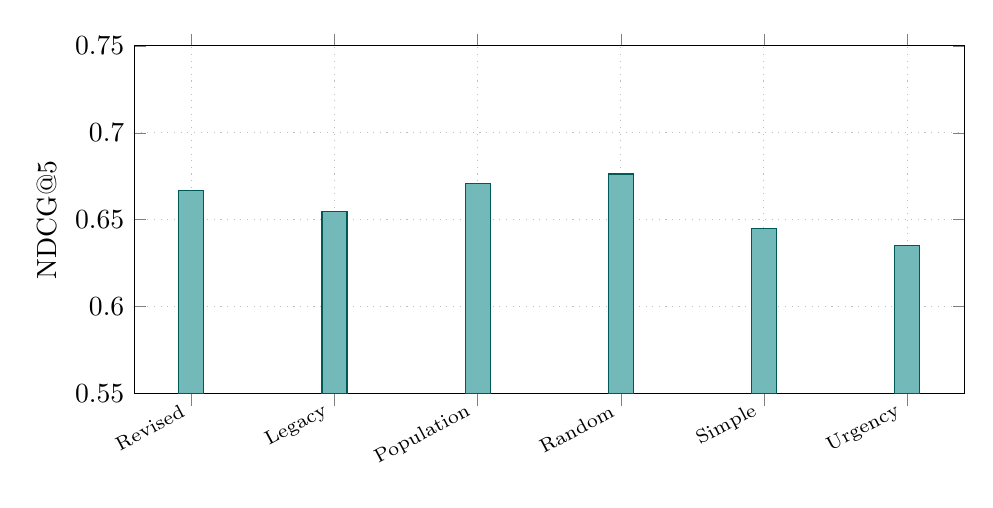
\begin{tikzpicture}
\begin{axis}[
  width=\textwidth,
  height=6.0cm,
  ybar,
  bar width=9pt,
  symbolic x coords={Revised,Legacy,Population,Random,Simple,Urgency},
  xtick=data,
  xticklabel style={font=\scriptsize,rotate=28,anchor=east},
  ylabel={NDCG@5},
  ymin=0.55,
  ymax=0.75,
  ytick={0.55,0.60,0.65,0.70,0.75},
  grid=major,
  grid style={dotted,gray!50},
  enlarge x limits=0.08,
]
\addplot+[fill=teal!55,draw=teal!70!black]
  coordinates {
    (Revised,0.6669)
    (Legacy,0.6548)
    (Population,0.6709)
    (Random,0.6763)
    (Simple,0.6448)
    (Urgency,0.6352)
  };
\end{axis}
\end{tikzpicture}
\caption{RQ2 alignment comparison across the candidate-4.1 policies. The
revised score is not above the random or population-only comparators; bootstrap
intervals are retained in the RQ2 summary artifact.}
\label{fig:rq2-ndcg}
\end{figure}

RQ3 reaches the same operational caution. On the Product partition, revised
versus legacy has harm effect $-14.34$ (Holm $p=.675$) and deadline effect
$+.0188$ (Holm $p=.160$), so no general improvement is established. Revised
is significantly worse than nearest-first on both harm and deadline, while
its advantage over FIFO is a comparison with a weak baseline. Product is
also worse than oracle under the revised policy and worse than matched-density
Additive on harm. Clustering errors thus propagate into dispatch outcomes.

\begin{figure}[t]
\centering
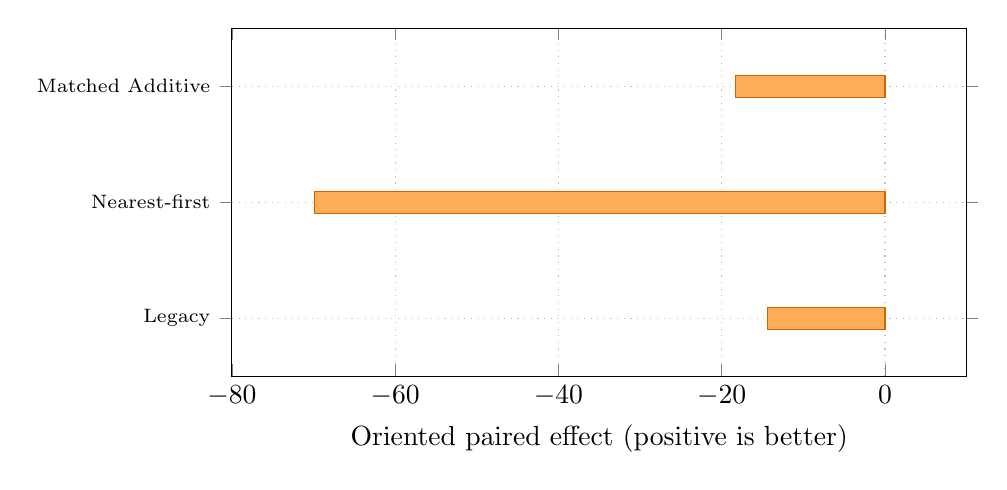
\begin{tikzpicture}
\begin{axis}[
  width=0.90\textwidth,
  height=6.0cm,
  xbar,
  bar width=8pt,
  symbolic y coords={Legacy,Nearest-first,Matched Additive},
  ytick=data,
  yticklabel style={font=\scriptsize},
  xlabel={Oriented paired effect (positive is better)},
  xmin=-80,
  xmax=10,
  xtick={-80,-60,-40,-20,0},
  grid=major,
  grid style={dotted,gray!50},
  enlarge y limits=0.25,
  ]
  \addplot+[fill=orange!65,draw=orange!80!black]
    coordinates {(-14.34,Legacy) (-69.88,Nearest-first) (-18.34,Matched Additive)};
\end{axis}
\end{tikzpicture}
\caption{RQ3 Product-partition harm effects for the revised policy. Negative
values indicate higher harm than the comparator; the values are taken from
the oriented paired-comparison results.}
\label{fig:rq3-harm}
\end{figure}

\section{Discussion and Threats to Validity}

The results separate mathematical safeguards from empirical utility. Product
gating supplies a finite edge bound in its positive-threshold domain, but the
independently tuned product pipeline does not outperform additive clustering.
The revised score removes exact-duplicate inflation, yet its ranking is not
better than simple comparators in general and can amplify coordinated
high-confidence campaigns. Dispatch outcomes confirm that a bounded score
cannot substitute for a validated operational objective.

All reports, incidents, and relevance signals are synthetic. RQ1 varies seeds
within generator 3.0.0; RQ2/RQ3 use a separate candidate-4.1 bundle. Neither
tests mechanism-shift OOD transfer or field performance. RQ1 does not provide
an empirical missingness test because all evaluated reports contain the four
core attributes. No expert panel validated weights, caps, or utility, and no
result measures extraction accuracy, device latency, memory, energy,
provenance authenticity, or model accuracy. A prospective mobile deployment
is therefore only an architecture proposal.

\section{Artifact and Conclusion}

The result folders contain the RQ1 summary and paired comparisons, RQ2/RQ3
CSVs, and SHA manifests for the candidate bundle. The manuscript treats
these CSVs as the numerical source of truth; the obsolete
\texttt{paper/short\_results.tex} and generated snapshots are not imported.
Before submission, the Colab audit must record the candidate source files,
priority configuration, and bundle hash, and every number in this paper must
trace to a current CSV row.

In conclusion, the study establishes conditional graph bounds and documents
competitive within-generator clustering, exact-duplicate invariance, and
several important negative results. It does not establish ranking alignment,
dispatch benefit, misinformation robustness, policy validity, or deployment
readiness. The contribution is an auditable stress-test boundary around those
claims, not a validated rescue policy.

\bibliographystyle{splncs04}
\bibliography{references}

\end{document}
